\chapter{Sistema Lineales}

\section{State-space systems}
We will focus on systems that can be described by quantifiable characteristics or states, e.g., temperature, velocity or voltage. These states might change over time. One might interact with a system via a quantifiable input, and one might measure some information from the states of the system via a quantifiable output.

Let us define $x(t)\in\mathbb{R}^n$, $y(t)\in\mathbb{R}^m$ and $u(t)\in\mathbb{R}^k$ as the stacked vector of states, the output, and the input of a system $\Sigma$ respectively. In particular, we will describe them as continuous signals over time, e.g., $x :[0,\infty) \to \mathbb{R}^n$. 

The system $\Sigma$ is a model that predicts the value of the states and the output over time. This prediction incorporates the impact of the input on the states and the output as well. We utilize differential equations as a tool to predict the evolution of the states of the system $\Sigma$ over time as follows
\begin{equation}
	\Sigma := \begin{cases}
		\dot x(t) =& f(x(t),u(t)) \\ y(t) =& g(x(t),u(t))
	\end{cases}, \nonumber
\end{equation}
where $\dot x := \frac{\mathrm{d}}{\mathrm{dt}}(x(t))$ is the short notation for total derivative with respect to time, and $f: \mathbb{R}^n \times \mathbb{R}^k \to \mathbb{R}^n$ and $g: \mathbb{R}^n \times \mathbb{R}^k \to \mathbb{R}^m$ are functions.

We can represent the system $\Sigma$ as a block with input/output ports as in figure \ref{fig: sigma}.

\begin{figure}[!h]
\centering
\begin{tikzpicture}[auto, node distance=2cm,>=latex']
	\node [input, name=input] {};
	\node [block, right of=input] (system) {$\Sigma$};
	\node [output, right of=system] (output) {};
	\draw [draw,->] (input) -- node {$u(t)$} (system);
	\draw [->] (system) -- node [name=y] {$y(t)$}(output);
\end{tikzpicture}
	\caption{Input/output block diagram of system $\Sigma$.}
	\label{fig: sigma}
\end{figure}

\subsection{Exercise: Inverted pendulum}

Derive the equations of motion of the mass in the inverted pendulum system in figure \ref{fig: invpen} as a first step to figure out the system's functions $f$ and $g$. Consider that we can interact with the system with a torque $T$ applied on the base, the mass is under a friction force proportional to its speed, and we can only measure the angle $\theta$ from the system.

\begin{figure}[!h]
\centering
	\includegraphics[scale=0.1]{./figuras/invpen.png}
	\caption{Inverted pendulum}
	\label{fig: invpen}
\end{figure}


\section{Linear maps}

In this chapter, we focus on a particular class of state-space systems called \emph{state-space linear systems}. First, we need the notion of \emph{linear map}.

\begin{definition} Consider the mapping $H: V \to W$. If $H$ preserves the operations of addition and scalar multiplication, i.e.,
\begin{align}
	H(v_1+v_2) &= H(v_1) + H(v_2), \quad v_1, v_2\in\mathbb{V} \nonumber \\
	H(\alpha v_1) &= \alpha H(v_1), \quad \alpha\in\mathbb{K} \nonumber,
\end{align}
then $H$ is a linear map.
\end{definition}

\subsection{Exercise: Check whether the following maps are linear or not}

\begin{enumerate}
	\item $H_1(v) := Av, A\in\mathbb{R}^{n\times n}, \quad v\in\mathbb{R}^n$
	\item $H_2(v) := \frac{\mathrm{d}}{\mathrm{dt}}(v(t)), \quad v\in\mathcal{C}^1$
	\item $H_3(v) := \int_0^T v(t) dt, \quad v\in\mathcal{C}^1, T\in\mathbb{R}_{\geq 0}$
	\item $H_4(v) := D(v) := v(t - T), \quad v\in\mathcal{C}^1, T\in\mathbb{R}_{\geq 0}$
	\item $H_5(v) := Av + b, \quad A\in\mathbb{R}^{n\times n}, v,b\in\mathbb{R}^n$
\end{enumerate}

\section{Continuous state-space linear systems}

The following system defines a continuous state-space linear system

\begin{equation}
	\Sigma := \begin{cases}
	\dot x(t) &= A(t)x(t) + B(t)u(t), \quad x\in\mathbb{R}^n, u\in\mathbb{R}^k \\
	\dot y(t) &= C(t)x(t) + D(t)u(t), \quad y\in\mathbb{R}^m
	\end{cases}
	\label{eq: linsys}
\end{equation}

\subsection{Exercise: Write as a block diagram the continuous state-space linear system and check that consists only of linear maps}

\subsection{Exercise: Interconnections of continuous state-space linear systems}
Rewrite as a single system, i.e., as in (\ref{eq: linsys}):

\begin{enumerate}
	\item the series (or cascade) interconnection of two continuous state-space linear systems, i.e., $y_1(t) = u_2(t)$.
	\item the parallel interconnection of two continuous state-space linear systems, i.e., $y(t) = y_1(t) + y_2(t)$.
	\item the feedback interconnection, i.e., $u_1(t) = u(t) - y(t)$, assuming $u, y, \in\mathbb{R}^k$.
\end{enumerate}

\begin{figure}
\centering
\begin{tikzpicture}[auto, node distance=3.5cm, >=latex']
	\node [input, name=input] {};
	\node [block, right of=input] (system) {$\Sigma_1$};
	\node [output, right of=system] (output) {};
	\draw [draw,->] (input) -- node {$u(t) = u_1(t)$} (system);
	\draw [->] (system) -- node [name=y] {$y_1(t)$}(output);
	\node [block, right of=output] (system2) {$\Sigma_2$};
	\node [output, right of=system2] (output2) {};
	\draw [draw,->] (output) -- node {$u_2(t)$} (system2);
	\draw [->] (system2) -- node [name=y] {$y_2(t) = y(t)$}(output2);
\end{tikzpicture}
	\caption{Example of series interconnection.}
	\label{fig: series}
\end{figure}

\section{Linearization of state-space systems}
Unfortunately, it is really (really) hard to calculate the analytic solution of $x(t)$ and $y(t)$ for a generic system $\Sigma$. Nevertheless, we will see on week 15 that we can find the analytic solution for a state-space linear system.

The question then is whether we can relate a generic $\Sigma$ to a state-space linear system.

If $f(x,t)$ and $g(x,t)$ are real analytic around a specific point $(x^*,u^*)$, then we can approximate them around $(x^*,u^*)$ by a Taylor series expansion. This approximation is what we call \emph{linearization} if we stop at order one in the Taylor series
\begin{equation}
	\Sigma := \begin{cases}
		\dot x(t) =& f(x(t),u(t)) \\ y(t) =& g(x(t),u(t))
	\end{cases} \approx
	\begin{cases}
	\dot x(t) &= A(t)x(t) + B(t)u(t) \\
	\dot y(t) &= C(t)x(t) + D(t)u(t)
\end{cases}  \quad x\approx x^*, u\approx u^*, \nonumber
\end{equation}
where
\begin{align}
	A(t) &= \begin{bmatrix}
		\frac{\partial f_1}{\partial x_1} & \dots & \frac{\partial f_1}{\partial x_n} \\
		\vdots & \vdots & \vdots \\
		\frac{\partial f_n}{\partial x_1} & \dots & \frac{\partial f_n}{\partial x_n}
	\end{bmatrix}_{|_{x=x^*, u=u^*}} \nonumber \\
	B(t) &= \begin{bmatrix}
		\frac{\partial f_1}{\partial u_1} & \dots & \frac{\partial f_1}{\partial u_k} \\
		\vdots & \vdots & \vdots \\
		\frac{\partial f_k}{\partial u_1} & \dots & \frac{\partial f_k}{\partial u_k}
	\end{bmatrix}_{|_{x=x^*, u=u^*}} \nonumber \\
	C(t) &= \begin{bmatrix}
		\frac{\partial g_1}{\partial x_1} & \dots & \frac{\partial g_1}{\partial x_n} \\
		\vdots & \vdots & \vdots \\
		\frac{\partial g_m}{\partial x_1} & \dots & \frac{\partial g_m}{\partial x_n}
	\end{bmatrix}_{|_{x=x^*, u=u^*}} \nonumber \\
	D(t) &= \begin{bmatrix}
		\frac{\partial g_1}{\partial u_1} & \dots & \frac{\partial g_1}{\partial u_k} \\
		\vdots & \vdots & \vdots \\
		\frac{\partial g_m}{\partial u_1} & \dots & \frac{\partial g_m}{\partial u_k}
	\end{bmatrix}_{|_{x=x^*, u=u^*}} \nonumber
\end{align}
Roughly speaking, we calculate the sensitivity (up to first order) of $f$ and $g$ when we make a small variation on $x$ and $u$ around $(x^*,u^*)$. How close $(x,u)$ must be to $(x^*,u^*)$ depends on the particular system $\Sigma$.
Recall that
\begin{equation}
	f = \begin{bmatrix}f_1 \\ f_2 \\ \vdots \\ f_n \end{bmatrix}, \quad
	g = \begin{bmatrix}g_1 \\ g_2 \\ \vdots \\ g_m \end{bmatrix} \nonumber,
\end{equation} and you can exploit the following identity when you have high order derivatives for some elements of $x$
\begin{equation}
	\begin{bmatrix}
	\dot q \\ \ddot q
	\end{bmatrix}
	=
	\begin{bmatrix}
	0 & 1 \\
	\ast & \ast
	\end{bmatrix}
	\begin{bmatrix}
	q \\ \dot q
	\end{bmatrix}, \nonumber
\end{equation}
so it is trivial to calculate some of the rows of $A$.

\section{Simulations / Numerical solutions}
We can still calculate numerical solutions (also known as simulations) for $\Sigma$ given a starting point $x(0)$. The \emph{Euler integration} is an easy numerical method that can give us some information about $\Sigma$. The following algorithm is what you can use in your Python/Matlab simulations
\begin{algo}
	\begin{enumerate}
		\item Set step time $\Delta T$
		\item Set $x = x(0)$
		\item Set $y = g(x,u)$
		\item Log $x$ and $y$, so you can plot them later
		\item Set $t = 0$
		\item Set final time $T^*$
		\item While $t \leq T^*$ then:
			\begin{enumerate}
				\item Set $x_{\text{new}} = x_{\text{old}} + f(x_{\text{old}},u)\Delta T$
				\item Set $y_{\text{new}} = g(x_{\text{new}},u)$
				\item Draw $x$
				\item Log $x$ and $y$, so you can plot them later
				\item Set $t = t + \Delta t$
			\end{enumerate}
		\item Plot the log for the elements of $x$ and $y$ over time $t$
	\end{enumerate}
\end{algo}
This algorithm performs okei when $\Delta T$ is sufficiently small. How small? It always depends on the system $\Sigma$, in particular, of $f$. Check \url{https://en.wikipedia.org/wiki/Euler_method} for more details, and of course, for more accurate methods. There are always compromises, typically good accuracy entails more computational cost per iteration.

For now, in the simulation we will leave $u = 0$, i.e., no control action over the system $\Sigma$. Once we know how to design $u$, we will calculate $u$ before the step 7.a in Algorithm 1.

\subsection{Inverted pendulum}
\begin{figure}[!h]
\centering
	\includegraphics[scale=0.1]{./invpen.png}
	\caption{Inverted pendulum}
	\label{fig: invpen}
\end{figure}

The dynamics of the inverted pendulum are given by
\begin{equation}
	\ddot\theta = \frac{1}{ml^2}\left(mgl\sin{\theta}-b\dot\theta + T\right). \nonumber
\end{equation}
Set the initial conditions $x(0) = \begin{bmatrix}\theta(0) \\ \dot\theta(0) \end{bmatrix}$ for the initial angle and initial angular velocity, and we set $u(t) = T = 0$ for now. The step 7.a in Algorithm 1 would be calculated sequentially by
\begin{align}
	\text{Set} \quad \dot\theta_{\text{new}} &= \dot\theta_{\text{old}} + \ddot\theta \Delta T \nonumber \\
	\text{Set} \quad \theta_{\text{new}} &= \theta_{\text{old}} + \dot\theta_{\text{new}} \Delta T. \nonumber
\end{align}

A Python simulation can be found at \url{https://github.com/noether/aut_course}.

\section{Solution to Linear State-Space systems}
The solution to an \emph{ordinary differential equation} (ODE) is given by the addition of two terms: the solution to the homogeneous part, and a particular solution to the non-homogeneous.

\begin{equation}
	\dot x(t) = \underbrace{A(t)x(t)}_{\text{homogeneous}} + \underbrace{B(t)u(t)}_{\text{non-homogeneous}}
	\label{eq: xdyn}
\end{equation}

\begin{theorem}{Peano-Barker series}
The unique solution to the homogeneous $\dot x = Ax$ is given by
	\begin{equation}
		x(t) = \Phi(t,t_0)x(t_0), \quad x(t_0)\in\mathbb{R}^n, t\geq 0,
	\end{equation}
where
	\begin{align}
		\Phi(t,t_0) := I + \int_{t_0}^t A(s_1)ds_1 + \int_{t_0}^t A(s_1) \int_{t_0}^{s_1} A(s_2)ds_2ds_1 \nonumber \\ + \int_{t_0}^t A(s_1) \int_{t_0}^{s_1} A(s_2)\int_{t_0}^{s_2} A(s_3) ds_3ds_2ds_1 + \dots . \label{eq: ser}
	\end{align}
\end{theorem}
Sketch of the proof:
First we calculate the following time derivative
	\begin{align}
		\frac{d}{dt}\Phi(t,t_0) &= A(t) + A(t)\int_{t_0}^{t}A(s_2)ds_2 \nonumber \\ &+ A(t)\int_{t_0}^t A(s_2) \int_{t_0}^{s_2} A(s_3)ds_3ds_2 + \dots \nonumber \\
		&= A(t) \Phi(t,t_0).
	\end{align}
We claim that the solution to the homogenenous part of (\ref{eq: xdyn}) is $x(t) = \Phi(t,t_0)x_0$ ($x_0$ is the short notation for $x(t_0)$), whose time derivative is given by
\begin{align}
	\frac{d}{dt} x &= \frac{d}{dt}\Phi(t,t_0)x_0 \nonumber \\
	&= A(t) \Phi(t,t_0) x_0 \nonumber \\
	&= A(t)x(t),
\end{align}
which is proving the identity $\dot x = A(t)x(t)$ given that $x(t) = \Phi(t,t_0)x_0$. In order to make this proof complete, we would need to prove that the series (\ref{eq: ser}) converges for $t\geq t_0$. That material should be covered in a standard course on differential equations.

The matrix $\Phi(t,t_0)$ is called the \textbf{\emph{state transition matrix}}. Given an initial condition $x_0$, we can predict $x(t)$ in (\ref{eq: xdyn}) by \emph{iterating} over and over with $\Phi(t,t_0)$ given that we do not interact with the system, i.e., $u(t) = 0, t\geq t_0$.

\subsection{Exercise}
Check that 
\begin{align}
	x(t) &= \Phi(t,t_0)x_0 + \int_{t_0}^t \Phi(t,\tau)B(\tau)u(\tau)d\tau \nonumber \\
	y(t) &= C(t)\phi(t,t_0)x_0 + \int_{t_0}^t C(t)\Phi(t,\tau)B(\tau)u(\tau)d\tau + D(t)u(t) \nonumber
\end{align}
are the solutions to

\begin{align}
	\dot x(t) &= A(t)x(t) + B(t)u(t)  \nonumber \\
	\dot y(t) &= C(t)x(t) + D(t)u(t)  \nonumber
\end{align}

\section{Solution to Linear Time Invariant Systems}

The matrix $\Phi(t,t_0)$ can be calculated analytically when $A$ is a matrix with constant coefficients. If $A$ is constant, we can take it out from the integrals in (\ref{eq: ser})
\begin{align}
	\Phi(t,t_0) := I + A \int_{t_0}^t ds_1 + A^2 \int_{t_0}^t \int_{t_0}^{s_1} ds_2ds_1 \nonumber \\ + A^3 \int_{t_0}^t \int_{t_0}^{s_1} \int_{t_0}^{s_2} ds_3ds_2ds_1 + \dots \label{eq: phi},
\end{align}
and noting that the following integrals can be easily solved
\begin{align}
	\int_{t_0}^t ds_1 &= (t-t_0) \nonumber \\
	\int_{t_0}^t\int_{t_0}^{s_1} ds_2ds_1 &= \frac{(t-t_0)^2}{2} \nonumber \\
	\vdots \nonumber \\
	\int_{t_0}^t\int_{t_0}^{s_1} \cdots \int_{t_0}^{s_{k-2}}\int_{t_0}^{s_{k-1}}ds_k ds_{k-1} \cdots ds_2ds_1 &= \frac{(t-t_0)^k}{k!}, \nonumber
\end{align}
then we have that (\ref{eq: phi}) can be calculated by
\begin{equation}
	\Phi(t,t_0) = \sum_{k=0}^{\infty} \frac{(t-t_0)^k}{k!}A^k,
\end{equation}
which resembles to the power series of the scalar exponential function, i.e., $e^x := \sum_{k=0}^{\infty}\frac{1}{k!}x^k = 1 + x + \frac{x^2}{2} + \frac{x^3}{3!} + \dots $. In fact, the definition of the \emph{exponential of a matrix} is
\begin{equation}
	exp(A) = I + A + \frac{1}{2} A^2 + \frac{1}{3!} A^3 + \dots
\end{equation}

Let us set $t_0 = 0$ for the sake of convinience, then
\begin{align}
	\Phi(t,0) &= I + tA + \frac{t^2}{2} A^2 + \frac{t^3}{3!} A^3 + \dots \nonumber \\
	&= exp(At),
\end{align}
therefore the solution to the homogeneous (\ref{eq: xdyn}) with $A$ constant and setting $t_0 = 0$ is
\begin{equation}
	x(t) = exp(At)x_0,\quad t\geq 0.
	\label{eq: xexp}
\end{equation}

To continue further, we need the following result from Linear Algebra.
\begin{theorem}
\textbf{Jordan Form}. For every square matrix $A\in\mathbb{C}^{n \times n}$, there exists a non-singular change of basis matrix $P\in\mathbb{C}^{n \times n}$ that transform $A$ into
\begin{equation}
	J = PAP^{-1} = \begin{bmatrix}
		J_1 & 0 & 0 & \dots & 0 \\
		0 & J_2 & 0 & \dots & 0 \\
		0 & 0 & J_3 & \dots & 0 \\
		\vdots & \vdots & \vdots & \cdots & \vdots \\
		0 & 0 & 0 & \cdots & J_l
	\end{bmatrix},
\end{equation}
where each $J_i$ is a Jordan block of the form
	\begin{equation}
	J_i = \begin{bmatrix}
\lambda_i & 1 & 0 & \dots & 0 \\
		0 & \lambda_i & 1 & \dots & 0 \\
		0 & 0 & \lambda_i & \dots & 0 \\
		\vdots & \vdots & \vdots & \cdots & \vdots \\
		0 & 0 & 0 & \cdots & \lambda_i
	\end{bmatrix}_{n_i\times n_i},
	\end{equation}
	where each $\lambda_i$ is an eigenvalue of $A$, and the number $l$ of Jordan blocks is equal to the total number of independent eigenvectors of $A$. The matrix $J$ is unique up to a reordering of the Jordan blocks and is called the \textbf{Jordan normal form} of $A$.
\end{theorem}

Note that $A = P^{-1}JP$ as well, and we leave as an exercise to prove that
\begin{equation}
	A^k = P^{-1} J^k P,
\end{equation}
so we can calculate
\begin{align}
	exp(At) &= P^{-1}\left(\sum_{k=1}^\infty \frac{t^k}{k!} \begin{bmatrix}J_1^k & 0 & \cdots & 0 \\ 0 & J_2^k & \cdots & 0 \\ \vdots & \vdots & \cdots & \vdots \\ 0 & 0 & \cdots & J_l^k \end{bmatrix} \right) P \nonumber \\
		&= P^{-1} \begin{bmatrix}exp(J_1t) & 0 & \cdots & 0 \\ 0 & exp(J_2t) & \cdots & 0 \\ \vdots & \vdots & \cdots & \vdots \\ 0 & 0 & \cdots & exp(J_lt) \end{bmatrix} P
\end{align}


Therefore if $J$ is just a diagonal matrix with the eigenvalues of $A$, i.e., $J_l = \lambda_l \in \mathbb{C}$, then $exp(J_lt) = e^{\lambda_lt} \in\mathbb{C}$ is a trivial calculation.

Now, let us check the consequencues on the following two conditions
\begin{enumerate}
	\item $J$ is diagonal.
	\item All the eigenvalues of $A$ have negative real part.
\end{enumerate}

Knowing that $\lim_{t\to\infty} e^{\lambda t} \to 0$ if $\lambda \in \mathbb{R}_{<0}$, then we will have that $exp(At) \to 0$ as $t\to\infty$ if the previous two conditions are satisfied! So if we take a look at (\ref{eq: xexp}), we can conclude that
\begin{equation}
	\lim_{t\to\infty} x(t) \to 0,
	\label{eq: xlim}
\end{equation}
therefore we can make a prediction on the evolution of $x(t)$ by just checking the eigenvalues of $A$. If $J$ is not diagonal we can also conclude similar results, but we will not cover them here. We will talk about stability in the next lecture, and how to design a controller such that we can guarantee (\ref{eq: xlim}).

\section{Guideline to design a linear controller for the inverted pendulum}
1. \\ \\
Given the model $\Sigma$ of a dynamical system
\begin{equation}
	\Sigma := \begin{cases}
		\dot x(t) =& f(x(t),u(t)) \\ y(t) =& g(x(t),u(t))
	\end{cases}, \nonumber
\end{equation}
choose an operational/equilibrium point $x^*$ of interest. \\

\textcolor{blue}{For the pendulum, let us choose when it is in vertical position and at rest, i.e., $\theta^* = 0$, $\dot\theta^* = 0$. So you we have that $x^* = \begin{bmatrix}0 \\ 0\end{bmatrix}$.} \\

2. \\ \\
Since $x^*$ is an equilibrium, find out which $u^*$ makes $\dot x(t) = 0$, i.e., $f(x^*,u^*) = 0$. \\
\textcolor{blue}{We have that $u = T$, and that $\ddot\theta = \frac{1}{ml^2}\left(mgl\sin\theta - b\dot\theta + T\right)$. To keep $x^*$ fixed, we need to set $\ddot\theta = 0$, therefore $u^* = T^* = 0$. Note that for another $x^*$, we would have different $T^*$.} \\

3. \\ \\
Now we want the system around $x^*$ and $u^*$ to be an stable equilibrium, i.e., for a small deviation/disturbance $\delta x$, we need to calculate the necessary $\delta u$ to keep the system at $x^*$.

We calculate the dynamics of $\delta x$ and $\delta u$, i.e., we linearize $\Sigma$ around $x^*$ and $u^*$.
\begin{equation}
	\Sigma := \begin{cases}
		\dot x(t) =& f(x(t),u(t)) \\ y(t) =& g(x(t),u(t))
	\end{cases} \approx
	\begin{cases}
		\dot {\delta x(t)} &= A(t) \delta x(t) + B(t) \delta u(t) \\
		\dot {\delta y(t)} &= C(t) \delta x(t) + D(t) \delta u(t)
	\end{cases} \quad \text{if } x\approx x^* + \delta x, u\approx u^* + \delta u, \nonumber
\end{equation}
where the matrices $A(t), B(t), C(t)$ and $D(t)$ are the Jacobians from Week 14. Note that it is usual to set the origin of the coordinates $x$ the system at $x^*$, this is why you will find in many places (including Week 14) $\delta x = x$ for the linearized version of $\Sigma$. \\
\textcolor{blue}{The Jacobians for the inverted pendulum are
\begin{align}
	A &= \begin{bmatrix}0 & 1 \\ \frac{1}{ml^2}(mgl\cos\theta) & -\frac{b}{ml^2} \end{bmatrix} \nonumber \\
		B &= \begin{bmatrix}0 \\ 1 \end{bmatrix} \nonumber \\
		C &= \begin{bmatrix}1 & 0 \\ 0 & 1\end{bmatrix} \nonumber \\
		D &= \begin{bmatrix}0 \\ 0 \end{bmatrix}.
\end{align}
Note that $A$ has to be evaluated at $x^*$ (check the notes from Week 14). Therefore, for $\theta = 0$, we have that $A = \begin{bmatrix}0 & 1 \\ \frac{g}{l} & -\frac{b}{ml^2} \end{bmatrix}$.} We assume that $C = I$, i.e., we can measure all the elements from the state vector $x$.\\

4. \\ \\

Let us calculate the linear controller 
\begin{equation}
	\delta u = K\delta y, \label{eq: con}
\end{equation}
such that $x^*$ is stable. We substitute (\ref{eq: con}) in the linearized $\Sigma$ resulting in
\begin{align}
\dot {\delta x(t)} &= A(t) \delta x(t) + B(t) K\delta y \nonumber \\
	&= A(t) \delta x(t) + B(t) K C(t) \delta x(t) + K D(t) \delta u(t) \nonumber \\
	&= \left(A(t) + B(t) K C(t)\right) x(t) + K D(t) u(t) \label{eq: system2}
\end{align}
Consider that $D(t) = 0$, and $A(t)$ and $B(t)$ are constant matrices, i.e., their elements do not depend on time. Then, we can write (\ref{eq: system2}) as
\begin{align}
\dot{\delta x(t)} &= \left(A + BKC\right) x(t) \\
	&= M x(t). \label{eq: system}
\end{align}
Then, the linearized system $\Sigma$ is stable around $x^*$ under small disturbances if and only if $M$ has all its eigenvalues with negative real part (Week 15).
\textcolor{blue}{
	To have the addition $A+BKC$, we need $K$ with the appropriate dimensions. For $C = I$ we have that $K = \begin{bmatrix}k_{11} & k_{12}\end{bmatrix}$, so we have that
\begin{equation}
	M = A + KBC = \begin{bmatrix}0 & 1 \\ \frac{g}{l}+\frac{k_{11}}{ml^2} & -\frac{b}{ml^2}+\frac{k_{12}}{ml^2}\end{bmatrix} \label{eq: Mp}
\end{equation}
}


5. \\ \\

A matrix $M\in\mathbb{R}^{n\times n}$ has $n$ eigenvalues. The eigenvalues of $M$ can be calculated from the following determinant
\begin{equation}
	\operatorname{det}\{M - \lambda_{i} I\} = 0, \quad i\in\{1,\dots,n\}. \label{eq: det}
\end{equation}
For example, for a $2 \times 2$ matrix we have that $\operatorname{det}\{A\} = \begin{bmatrix}a_{11} & a_{12} \\ a_{21} & a_{22}\end{bmatrix} = a_{11}a_{22} - a_{12}a_{21}$. Therefore we have that (\ref{eq: det}) is
\begin{equation}
	(m_{11} - \lambda_i) (m_{22} - \lambda_i) - m_{12}m_{21} = 0, \quad  i\in\{1,2\}. \label{eq: con2}
\end{equation}
The values for the elements of $K$ are calculated by setting an arbitrary $\lambda_i < 0$. This solution is guaranteed for $C = I$ and $D = 0$. \\
\textcolor{blue}{
	We have that (\ref{eq: con2}) from $M$ in (\ref{eq: Mp}) is
\begin{equation}
	\lambda^2 + \lambda\left(\frac{1}{ml^2}(b-k_{12})\right) - \frac{g}{l}-\frac{k_{11}}{ml^2}, \nonumber
\end{equation}
whose solution is given by
\begin{equation}
	\lambda_{1,2} = \frac{-\frac{1}{ml^2}(b-k_{12}) \pm \sqrt{\frac{(b-k_{12})^2}{m^2l^4}+4(\frac{g}{l}+\frac{k_{11}}{ml^2})}}{2}. \label{eq: lc}
\end{equation}
Let us find some conditions for $k_{11}$ and $k_{12}$ such that we can guarantee that $\lambda_1$ and $\lambda_2$ are two real negative numbers. For example, if force
\begin{equation}
	k_{12} < b,
\end{equation}
then $-\frac{1}{ml^2}(b-k_{12})$ in (\ref{eq: lc}) is a negative number. Note that $b$ is a coefficient friction in the pendulum equation, therefore if $b = 1$, we can have $-\infty < k_{12} < 1$, i.e., the gain $k_{12}$ can be even positive as long as it is smaller than $b$. Now we turn our attention at the square root in (\ref{eq: lc}). Assume that we take the positive solution $r>0$ of the square root in (\ref{eq: lc}). Now we need to add or subtract $r$ to $-\frac{1}{ml^2}(b-k_{12})$. We note that for $\lambda_1$ if $-\frac{1}{ml^2}(b-k_{12})$ is negative then $-\frac{1}{ml^2}(b-k_{12})- r$ is still negative, so $\lambda_1 < 0$. For $\lambda_2$ we need to calculate $k_{11}$ such that  $-\frac{1}{ml^2}(b-k_{12}) + r < 0$. If we set $k_{11} < -gml$ then $\sqrt{\frac{(b-k_{12})^2}{m^2l^4}+4(\frac{g}{l}+\frac{k_{11}}{ml^2})} < \sqrt{\frac{(b-k_{12})^2}{m^2l^4}} = \frac{1}{ml^2}(b-k_{12})$. Therefore we guarantee that $r < \frac{1}{ml^2}(b-k_{12})$, thus $\lambda_2 < 0$. Note that $k_{11}$ not only needs to be negative but \emph{negative enough}. Check in the Python script the consequences of playing around these limits for $k_{11}$ and $k_{12}$.
}

\section{Controller for the inverted pendulum}
Design a controller for
\begin{align}
	x_1^* = \begin{cases}\theta^* &= 0 \\ \dot\theta^*&= 0 \end{cases} \nonumber \\
		x_2^* = \begin{cases}\theta^* &= \frac{\pi}{4} \\ \dot\theta^*&= 0 \end{cases}. \nonumber
\end{align}
We will first assume that we can measure $\theta$ and $\dot\theta$, i.e., $C = I$. Note that for $M = (A - BKC)$ with $C = I$ the dimensions of $K$ must be $1 \times 2$, i.e., $K = \begin{bmatrix}k_{11} & k_{12} \end{bmatrix}$. Note that in this case we have that $K\delta y = k_{11}\delta\theta + k_{12}\delta\dot\theta$. Remember that the input $u = u^* + \delta u$, and that for the pendulum $u = T$, i.e., the applied torque.

\textbf{The exercise asks to find the values $k_{11}$ and $k_{12}$ for two arbitrary negative real eigenvalues $\lambda_1$ and $\lambda_2$ in (\ref{eq: con2}).}

Simulate your designed controller in the Python script. Check that your $x^*$ are stable if you start close to them, and you can further check the robustness by applying small disturbances, e.g., add a small random number to $x$ at every iteration.

Is it possible to design a stable controller with $C = \begin{bmatrix}1 & 0\end{bmatrix}$? and for $C = \begin{bmatrix}0 & 1\end{bmatrix}$? Note that for this cases $K$ will have different dimensions than for $C = I$ since $C$ has different dimensions as well.



